% !TEX program = pdflatex
% =====================================================================
%  TwA Research Webinar — Emily's econ-audit segment (~18 min)
%  June 15, 2026.  Reframe of UVM Session 2 deck (Demo 2 centered).
%  Preamble matches Session2_Slides/session_2_slides.tex (shared design).
% =====================================================================
\documentclass[aspectratio=169, 10pt]{beamer}

%% ============================================================
%% PACKAGES
%% ============================================================
\usepackage[T1]{fontenc}
\usepackage{lmodern}
\usepackage{graphicx}
\usepackage{booktabs}
\usepackage{array}
\usepackage{tabularx}
\usepackage{colortbl}
\usepackage{tikz}
\usetikzlibrary{positioning, calc, arrows.meta, shapes.geometric, fit, shadows}
\usepackage[most]{tcolorbox}
\usepackage{fontawesome5}
\usepackage{hyperref}
\usepackage{multicol}
\usepackage{xcolor}
\usepackage{textcomp}
\usepackage{pifont}

\graphicspath{{figures/}}

%% ============================================================
%% COLOR DEFINITIONS
%% ============================================================
\definecolor{UVMGreen}{HTML}{154734}
\definecolor{UVMGold}{HTML}{D4A84B}
\definecolor{SlateTeal}{HTML}{1B4D5C}
\definecolor{DeepCharcoal}{HTML}{2C3E50}
\definecolor{SoftCoral}{HTML}{C0534D}
\definecolor{CoolGray}{HTML}{8899A6}
\definecolor{PaleSage}{HTML}{EDF2F0}
\definecolor{LightGold}{HTML}{FDF6E3}
\definecolor{DarkSlate}{HTML}{0F2B36}
\definecolor{AccentBlue}{HTML}{3498DB}

%% ============================================================
%% BEAMER THEME SETUP
%% ============================================================
\setbeamercolor{structure}{fg=SlateTeal}
\setbeamercolor{normal text}{fg=DeepCharcoal}
\setbeamercolor{frametitle}{fg=SlateTeal}
\setbeamercolor{title}{fg=SlateTeal}
\setbeamercolor{subtitle}{fg=UVMGold}
\setbeamercolor{author}{fg=DeepCharcoal}
\setbeamercolor{date}{fg=CoolGray}
\setbeamercolor{institute}{fg=CoolGray}
\setbeamercolor{footline}{fg=CoolGray}
\setbeamercolor{block title}{fg=white, bg=SlateTeal}
\setbeamercolor{block body}{bg=PaleSage}
\setbeamercolor{alerted text}{fg=SoftCoral}
\setbeamercolor{item}{fg=SlateTeal}
\setbeamercolor{subitem}{fg=CoolGray}

\setbeamerfont{title}{size=\Large, series=\bfseries}
\setbeamerfont{subtitle}{size=\normalsize}
\setbeamerfont{frametitle}{size=\large, series=\bfseries}
\setbeamerfont{footline}{size=\tiny}

\setbeamertemplate{navigation symbols}{}

% Custom frame title
\setbeamertemplate{frametitle}{%
  \vskip14pt%
  \nointerlineskip%
  {\usebeamerfont{frametitle}\usebeamercolor[fg]{frametitle}\insertframetitle\par}%
  \vskip2pt%
  {\color{UVMGold}\rule{\textwidth}{1.2pt}}%
  \vskip3pt%
}

% Custom footline
\setbeamertemplate{footline}{%
  \begin{beamercolorbox}[wd=\paperwidth, ht=16pt, right, rightskip=1.5cm]{footline}%
    \usebeamerfont{footline}\insertframenumber\,/\,\inserttotalframenumber\vskip3pt%
  \end{beamercolorbox}%
}

% Itemize styles
\setbeamertemplate{itemize item}{\color{SlateTeal}\raisebox{0.15ex}{\small$\blacktriangleright$}}
\setbeamertemplate{itemize subitem}{\color{CoolGray}\raisebox{0.1ex}{\footnotesize$\bullet$}}

% Compact tcolorbox defaults
\tcbset{
  keybox/.style={
    colback=PaleSage, colframe=SlateTeal, boxrule=0.8pt, arc=3pt,
    left=6pt, right=6pt, top=4pt, bottom=4pt,
    fonttitle=\bfseries\small\color{white}, coltitle=white, colbacktitle=SlateTeal,
  },
  accentbox/.style={
    colback=LightGold, colframe=UVMGold, boxrule=0.8pt, arc=3pt,
    left=6pt, right=6pt, top=4pt, bottom=4pt,
  },
  quotebox/.style={
    colback=PaleSage, colframe=SlateTeal!50, boxrule=0.5pt, arc=2pt,
    left=8pt, right=8pt, top=4pt, bottom=4pt,
    borderline west={3pt}{0pt}{UVMGold},
  },
  coralbox/.style={
    colback=SoftCoral!8, colframe=SoftCoral, boxrule=0.8pt, arc=3pt,
    left=6pt, right=6pt, top=3pt, bottom=3pt,
    fonttitle=\bfseries\small\color{white}, coltitle=white, colbacktitle=SoftCoral,
  },
}

%% ============================================================
%% METADATA
%% ============================================================
\title{AI as an Adversarial Reader}
\subtitle{Auditing Code and Papers Before You Submit}
\author{Emily Beam}
\institute{Thinking with Agents \;$\cdot$\; Research Webinar}
\date{June 15, 2026}

\usepackage{pgfplots}
\pgfplotsset{compat=newest}
\usetikzlibrary{backgrounds,patterns,decorations.pathreplacing}
\begin{document}

%% ====== WELCOME / TITLE ======
{
\setbeamertemplate{footline}{}
\begin{frame}[plain]
\begin{tikzpicture}[remember picture, overlay]
  \fill[SlateTeal] (current page.north west) rectangle (current page.south east);
  \fill[UVMGold] ([yshift=0.3cm]current page.center -| current page.west) rectangle ([yshift=0.25cm]current page.center -| current page.east);
  \node[anchor=center, text=white, font=\fontsize{28}{34}\bfseries\selectfont] at ([yshift=2.2cm]current page.center) {Thinking With Agents};
  \node[anchor=center, text=UVMGold, font=\fontsize{15}{20}\selectfont] at ([yshift=1.2cm]current page.center) {Webinar 1: AI for Research};
  \node[anchor=center, text=white, font=\large\bfseries] at ([yshift=-0.6cm]current page.center) {Emily Beam \quad\&\quad Erkmen G. Aslim};
  \node[anchor=center, text=PaleSage, font=\normalsize] at ([yshift=-1.3cm]current page.center) {University of Vermont \;$\cdot$\; Department of Economics};
  \node[anchor=center, text=CoolGray!70!white, font=\small] at ([yshift=-2.2cm]current page.center) {June 15, 2026 \quad$\cdot$\quad Live Online};
  \node[text=white, opacity=0.04, font=\fontsize{100}{100}\selectfont, anchor=center, rotate=-15] at ([xshift=5cm, yshift=1.5cm]current page.center) {\faRobot};
\end{tikzpicture}
\end{frame}
}


%% ====== HOW THIS WORKS (housekeeping) ======
\begin{frame}{How This Works}
\vskip2pt
\begin{columns}[T]
\begin{column}{0.48\textwidth}
\begin{tcolorbox}[keybox, title={\faComments\quad Questions}]
\small One of us presents while the other watches the chat. \textbf{Drop questions any time} --- we'll take them between blocks.
\end{tcolorbox}
\vskip4pt
\begin{tcolorbox}[keybox, title={\faVideo\quad Recording}]
\small We're \textbf{not} posting the full recording publicly (still figuring that out) --- but we'll share the generally useful bits.
\end{tcolorbox}
\end{column}
\begin{column}{0.48\textwidth}
\begin{tcolorbox}[accentbox, title={\faClipboardCheck\quad Afterward}, fonttitle=\bfseries\small]
\small We'll follow up with a short \textbf{survey}. We'd genuinely appreciate your feedback --- it shapes the bootcamp this is building toward.
\end{tcolorbox}
\vskip4pt
\begin{tcolorbox}[quotebox, top=3pt, bottom=3pt]
\small This is \textbf{mostly live}. Things may break --- that's part of the honest picture.
\end{tcolorbox}
\end{column}
\end{columns}
\end{frame}

% Figure: figures/audience_charts.png  (rendered from the survey memo).
\begin{frame}{Who's in the Room}
\vskip-4pt
\begin{center}
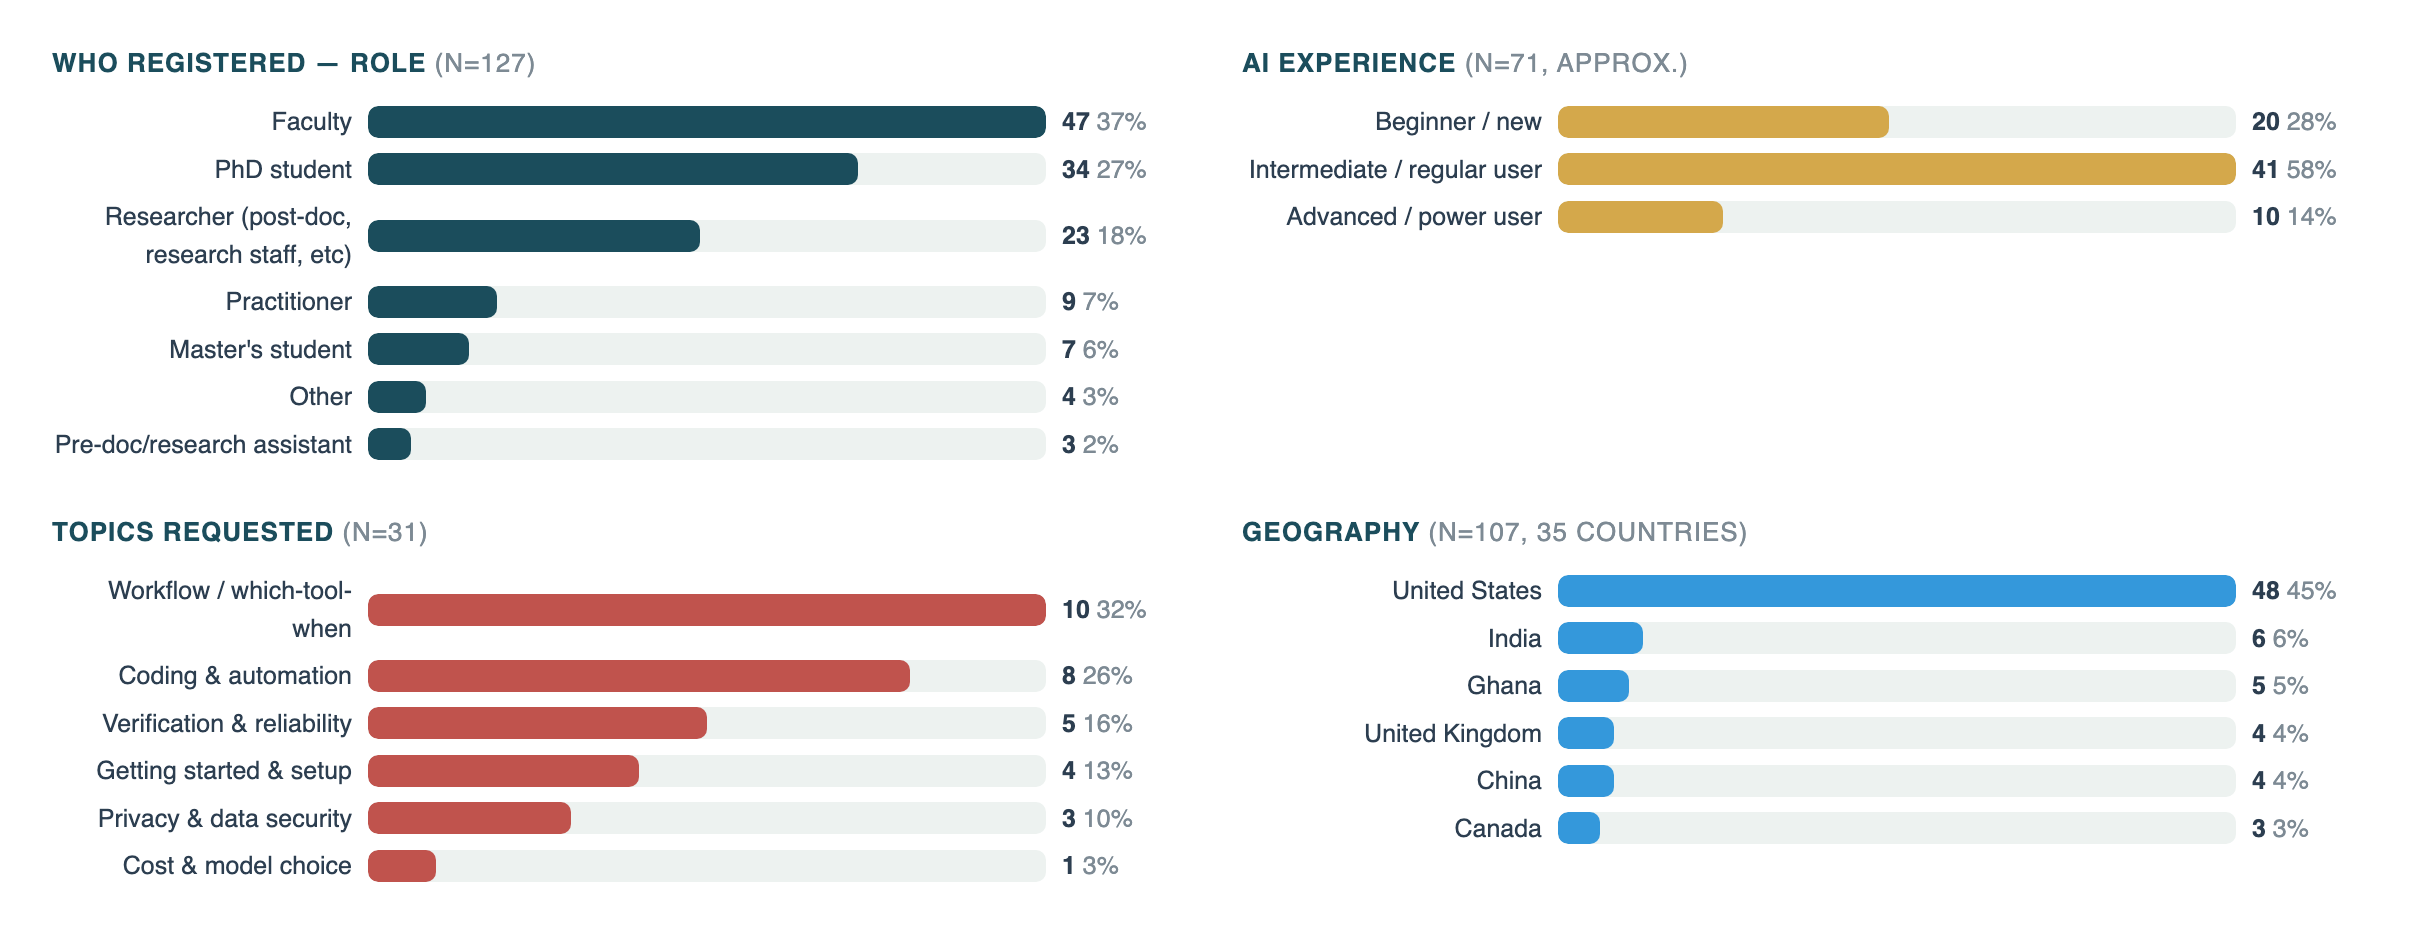
\includegraphics[width=\textwidth]{audience_charts.png}
\end{center}
%\vskip-2pt
%\begin{tcolorbox}[accentbox, halign=center, top=2pt, bottom=2pt]
%\small First-timers to daily power users, mostly international --- \textbf{this hour is built for all of you: orient first, then go deep.}
%\end{tcolorbox}
\end{frame}

%% ====== TODAY: THE ARC ======
\begin{frame}{Today: Two Hours, Two Halves}
\vskip2pt
\begin{columns}[T]
\begin{column}{0.48\textwidth}
\begin{tcolorbox}[keybox, title={\faCompass\quad Hour 1 --- Emily}]
\small
\begin{itemize}\setlength{\itemsep}{3pt}
  \item \textbf{Foundations:} what these tools are, which to reach for, how to start safely
  \item \textbf{Auditing your research:} AI as an adversarial reader of your code \& your paper
\end{itemize}
\end{tcolorbox}
\end{column}
\begin{column}{0.48\textwidth}
\begin{tcolorbox}[keybox, title={\faComments\quad Hour 2 --- Erkmen}]
\small
\begin{itemize}\setlength{\itemsep}{3pt}
  \item Ideas \& the verification mindset
  \item A website-builder demo (your CV $\rightarrow$ a live site)
  \item A live research brainstorm
\end{itemize}
\end{tcolorbox}
\end{column}
\end{columns}
\vskip8pt
\begin{tcolorbox}[accentbox, halign=center, top=3pt, bottom=3pt]
\small Mostly \textbf{live in the terminal}. Watch along --- drop questions in the chat; we'll take them between blocks.
\end{tcolorbox}
\end{frame}

%% ====== THIS HOUR: OUTLINE + PAYOFF SIGNPOST ======
\begin{frame}{My Hour, Roughly}
\vskip4pt
\begin{columns}[T]
\begin{column}{0.60\textwidth}
\begin{tcolorbox}[keybox, title={\faClock\quad The next 60 minutes}, top=3pt, bottom=3pt]
\small
\begin{itemize}\setlength{\itemsep}{5pt}
  \item \textbf{$\sim$10 min --- Orient:} what these tools are, which to reach for, how to start safely
  \item \textbf{$\sim$10 min --- A quick live demo:} teach it your writing voice
  \item \textbf{$\sim$30 min --- The payoff:} AI as an adversarial reader of your \textbf{code} and your \textbf{paper}
\end{itemize}
\end{tcolorbox}
\end{column}
\begin{column}{0.36\textwidth}
\begin{tcolorbox}[accentbox, top=3pt, bottom=3pt]
\small Not here to \textbf{sell} you on these tools --- you already signed up. Here to help you \textbf{start} and \textbf{trust} them.
\end{tcolorbox}
\vskip4pt
\begin{tcolorbox}[quotebox, top=3pt, bottom=3pt]
\scriptsize \textbf{Already fluent?} The research audit (\textasciitilde{}halfway in) is the part built for you.
\end{tcolorbox}
\end{column}
\end{columns}
\end{frame}

%% ====== SECTION DIVIDER: FOUNDATIONS ======
{
\setbeamertemplate{footline}{}
\setbeamercolor{background canvas}{bg=SlateTeal}
\begin{frame}[plain, noframenumbering]
\centering\vfill
{\fontsize{22}{28}\bfseries\selectfont\color{white} Part 1}\\[6pt]
{\color{UVMGold}\rule{5cm}{0.8pt}}\\[6pt]
{\normalsize\color{UVMGold} Foundations --- What These Tools Are \& How to Start}
\vfill
\end{frame}
}


%% ---- Three ways to interact: chat / IDE / agent ----
\begin{frame}{Three Ways to Work With AI}
\vskip2pt
\begin{columns}[T]
\begin{column}{0.31\textwidth}
\begin{tcolorbox}[colback=PaleSage, colframe=CoolGray, boxrule=0.6pt, arc=3pt, left=5pt, right=5pt, top=3pt, bottom=3pt, title={\faComments\quad 1. Chat window}, fonttitle=\bfseries\scriptsize, coltitle=DeepCharcoal, colbacktitle=PaleSage!80]
\scriptsize
{\color{CoolGray}\textit{ChatGPT / Claude web}}
\vskip3pt
\begin{itemize}\setlength{\itemsep}{1pt}
  \item Ask questions, paste text
  \item[\color{SoftCoral}\faTimes] Can't see your files
\end{itemize}
\vskip2pt
{\color{CoolGray} Like \textbf{texting a smart friend}.}
\end{tcolorbox}
\end{column}
\begin{column}{0.31\textwidth}
\begin{tcolorbox}[colback=PaleSage, colframe=CoolGray, boxrule=0.6pt, arc=3pt, left=5pt, right=5pt, top=3pt, bottom=3pt, title={\faCode\quad 2. In your editor}, fonttitle=\bfseries\scriptsize, coltitle=DeepCharcoal, colbacktitle=PaleSage!80]
\scriptsize
{\color{CoolGray}\textit{VS Code / Cursor}}
\vskip3pt
\begin{itemize}\setlength{\itemsep}{1pt}
  \item AI inside your IDE
  \item Sees the file you're in
  \item Autocomplete \& inline edits
\end{itemize}
\vskip2pt
{\color{CoolGray} Like a \textbf{co-pilot} as you type.}
\end{tcolorbox}
\end{column}
\begin{column}{0.34\textwidth}
\begin{tcolorbox}[colback=LightGold, colframe=UVMGold, boxrule=0.9pt, arc=3pt, left=5pt, right=5pt, top=3pt, bottom=3pt, title={\faTerminal\quad 3. Agent \;{\normalfont\itshape(today)}}, fonttitle=\bfseries\scriptsize, coltitle=DeepCharcoal, colbacktitle=LightGold!80]
\scriptsize
{\color{SlateTeal}\textit{Claude Code / Codex}}
\vskip3pt
\begin{itemize}\setlength{\itemsep}{1pt}
  \item[\color{SlateTeal}\faCheck] Reads \& edits your files
  \item[\color{SlateTeal}\faCheck] Runs commands
  \item[\color{SlateTeal}\faCheck] Works across a project
\end{itemize}
\vskip2pt
{\color{CoolGray} Like an \textbf{RA sitting next to you}.}
\end{tcolorbox}
\end{column}
\end{columns}
\vskip4pt
{\centering\scriptsize\color{CoolGray} The agent runs two ways: in your \textbf{terminal} (type \texttt{claude} / \texttt{codex}) or a \textbf{desktop app} --- terminal gets new features first; the app is friendlier to start.\par}
\vskip4pt
\begin{tcolorbox}[accentbox, halign=center, top=3pt, bottom=3pt]
\small All three are useful --- we'll focus on the \textbf{agent}, because it's the one that can do real research work end-to-end.
\end{tcolorbox}
\end{frame}

%% ---- bootcamp: Which tool economists use ----
\begin{frame}{Which Agentic Tool Are Economists Using?}
\centering
\vskip2pt
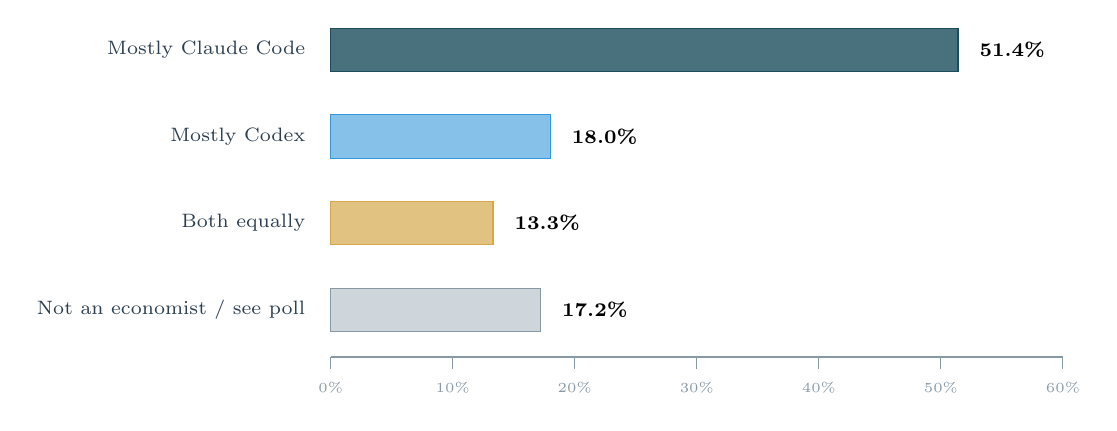
\begin{tikzpicture}[
  barlab/.style={font=\scriptsize, anchor=east, text=DeepCharcoal},
  pctlab/.style={font=\scriptsize\bfseries, anchor=west},
]
  % Y positions
  \def\ya{0}    % Not an economist
  \def\yb{1.1}  % Both equally
  \def\yc{2.2}  % Mostly Codex
  \def\yd{3.3}  % Mostly Claude Code
  \def\bh{0.55} % bar height
  \def\sc{0.155} % scale: 1% = 0.155cm

  % Labels
  \node[barlab] at (-0.2, \yd) {Mostly Claude Code};
  \node[barlab] at (-0.2, \yc) {Mostly Codex};
  \node[barlab] at (-0.2, \yb) {Both equally};
  \node[barlab] at (-0.2, \ya) {Not an economist / see poll};

  % Bars
  \fill[SlateTeal!80] (0, \yd-\bh/2) rectangle ({51.4*\sc}, \yd+\bh/2);
  \draw[SlateTeal] (0, \yd-\bh/2) rectangle ({51.4*\sc}, \yd+\bh/2);

  \fill[AccentBlue!60] (0, \yc-\bh/2) rectangle ({18.0*\sc}, \yc+\bh/2);
  \draw[AccentBlue] (0, \yc-\bh/2) rectangle ({18.0*\sc}, \yc+\bh/2);

  \fill[UVMGold!70] (0, \yb-\bh/2) rectangle ({13.3*\sc}, \yb+\bh/2);
  \draw[UVMGold] (0, \yb-\bh/2) rectangle ({13.3*\sc}, \yb+\bh/2);

  \fill[CoolGray!40] (0, \ya-\bh/2) rectangle ({17.2*\sc}, \ya+\bh/2);
  \draw[CoolGray] (0, \ya-\bh/2) rectangle ({17.2*\sc}, \ya+\bh/2);

  % Percentage labels (all outside bars, same style)
  \node[pctlab] at ({51.4*\sc + 0.15}, \yd) {51.4\%};
  \node[pctlab] at ({18.0*\sc + 0.15}, \yc) {18.0\%};
  \node[pctlab] at ({13.3*\sc + 0.15}, \yb) {13.3\%};
  \node[pctlab] at ({17.2*\sc + 0.15}, \ya) {17.2\%};

  % Axis line
  \draw[CoolGray] (0, -0.6) -- ({60*\sc}, -0.6);
  % Tick marks
  \foreach \v in {0,10,20,30,40,50,60} {
    \draw[CoolGray] ({\v*\sc}, -0.6) -- ({\v*\sc}, -0.75);
    \node[font=\tiny, text=CoolGray, anchor=north] at ({\v*\sc}, -0.8) {\v\%};
  }
\end{tikzpicture}
\vskip4pt
\pause
\begin{tcolorbox}[accentbox, width=12cm, halign=center]
\small The space is evolving fast. \textbf{Our recommendation:} there's value in using \textbf{both}.
\end{tcolorbox}
\vskip1pt
{\tiny\color{CoolGray} Source: @aniketapanjwani poll, X.com --- 459 votes, March 8, 2026}
\end{frame}

%% ---- bootcamp: Pricing / subscription ----
\begin{frame}{Pricing --- What Subscription Do You Need?}
\begin{columns}[T]
\begin{column}{0.47\textwidth}
\begin{tcolorbox}[keybox, title={\faDollarSign\quad Plans}]
\small
\textbf{Light user} (\$20/mo each):\\
Claude Pro + ChatGPT Plus\\[3pt]
\textbf{Heavy user:}\\
Claude Max: \$100--200/mo\\
ChatGPT Pro: \$200/mo\\[3pt]
\textbf{Pay-as-you-go (API):}\\
Claude Sonnet: \$3--15 per M tokens
\end{tcolorbox}
\end{column}
\begin{column}{0.47\textwidth}
\begin{tcolorbox}[accentbox]
\small
\textbf{Our recommendation:}
\vskip2pt
Start with the \textbf{\$20/month} plan. Play around before deciding to upgrade.
\vskip4pt
\textbf{Already have ChatGPT?}\\
Codex is included --- no-brainer to try.
\end{tcolorbox}
\vskip4pt
\begin{tcolorbox}[colback=PaleSage, colframe=CoolGray!50, boxrule=0.4pt, left=4pt, right=4pt, top=2pt, bottom=2pt]
\centering\small
\textbf{What's a token?} 1 token $\approx$ $\frac{3}{4}$ of a word.\\
200K tokens $\approx$ 150K words $\approx$ context limit.
\end{tcolorbox}
\end{column}
\end{columns}
\end{frame}

%% ---- bootcamp: Markdown output ----
\begin{frame}{Why It Hands You Plain Text (Markdown)}
\begin{columns}[T]
\begin{column}{0.44\textwidth}
\begin{tcolorbox}[keybox, title={\faFile\quad It writes in Markdown --- and that's a feature}, top=2pt, bottom=2pt]
\small
A \texttt{.md} file is just plain text. \textbf{You never edit the syntax} --- a viewer renders it for you.
\vskip3pt
Why plain text is the right default for research:
\begin{itemize}\setlength{\itemsep}{1pt}
  \item \textbf{Portable \& future-proof} --- opens anywhere, forever
  \item \textbf{Version-controllable} --- Git tracks every change
  \item \textbf{Converts on demand} --- \texttt{.docx}, \texttt{.pdf}, \texttt{.tex}, slides
\end{itemize}
\vskip2pt
{\scriptsize\color{CoolGray} Viewers: \href{https://obsidian.md}{Obsidian} (free) or Typora (\$15).}
\end{tcolorbox}
\end{column}
\begin{column}{0.52\textwidth}
\centering
{\small\bfseries\color{SlateTeal} A viewer renders it like this:}\\[4pt]
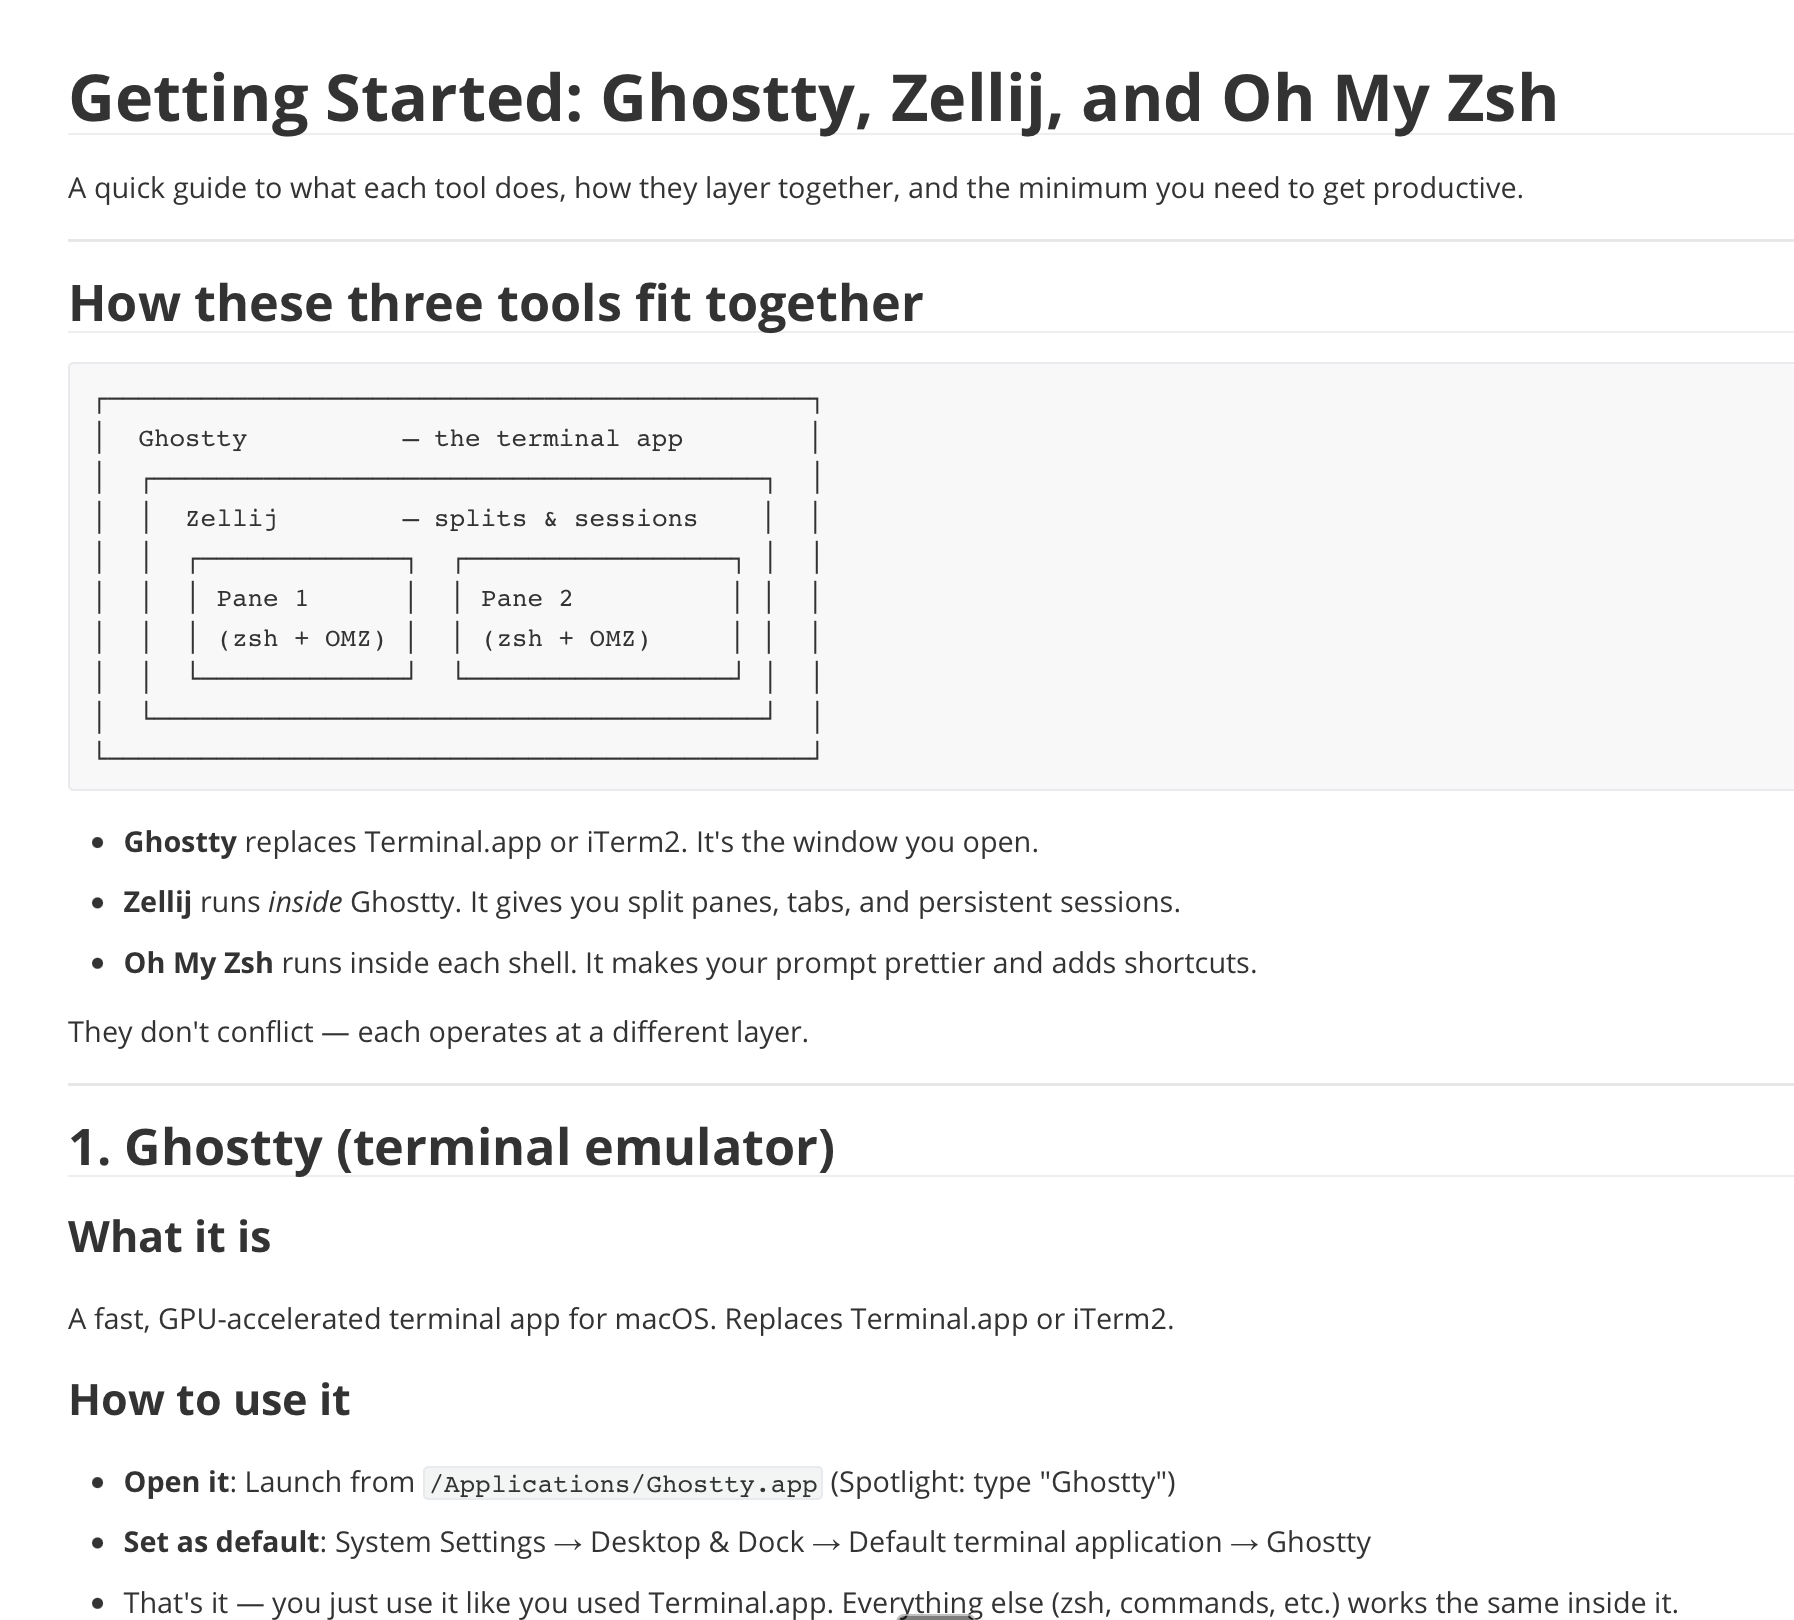
\includegraphics[width=\textwidth, height=0.6\textheight, keepaspectratio]{markdown-pretty.png}
\end{column}
\end{columns}
\end{frame}

%% ---- bootcamp: Context window ----
\begin{frame}{The Context Window --- The Key Concept}
\begin{columns}[T]
\begin{column}{0.47\textwidth}
\begin{tcolorbox}[keybox, title={What the model ``sees''}]
\small
\begin{itemize}\setlength{\itemsep}{0pt}
  \item System prompt
  \item Developer messages (tools)
  \item Your prompt + model's ``thinking''
  \item Tool calls \& results
  \item Model's response
  \item \ldots all appended each turn
\end{itemize}
\end{tcolorbox}
\end{column}
\begin{column}{0.47\textwidth}
\begin{tcolorbox}[accentbox]
\small
\textbf{Every turn:} the entire history gets sent as one input.
\vskip4pt
\textbf{Limit:} $\sim$200K tokens ($\sim$150K words), increaingly $\sim$ 1M tokens ($\sim$750k words)
\end{tcolorbox}
\vskip4pt
\pause
\begin{tcolorbox}[colback=SoftCoral!8, colframe=SoftCoral, boxrule=0.5pt, left=5pt, right=5pt, top=3pt, bottom=3pt]
\centering\small
This is the \textbf{single most important concept} for using these tools well.
\end{tcolorbox}
\end{column}
\end{columns}
\end{frame}

%% ---- bootcamp: Three rules for context ----
\begin{frame}{Three Rules for Context Management}
\begin{columns}[T]
\begin{column}{0.55\textwidth}
\vskip2pt
\begin{enumerate}\setlength{\itemsep}{6pt}
  \item[\color{SlateTeal}\textbf{1.}] \textbf{Long sessions degrade} --- after 20+ turns, start fresh (\texttt{/clear})
  \pause
  \item[\color{SlateTeal}\textbf{2.}] \textbf{Write ideas to files} --- files persist, context doesn't
  \pause
  \item[\color{SlateTeal}\textbf{3.}] \textbf{Break work into chunks} --- 5--10 turn focused sessions
\end{enumerate}
\vskip8pt
\begin{tcolorbox}[quotebox]
\small \textbf{Frequent intentional compaction is better} than hitting the wall and letting auto-compaction lose details.
\end{tcolorbox}
\end{column}
\begin{column}{0.42\textwidth}
\vskip2pt
\begin{tcolorbox}[accentbox]
\small
\textbf{The ``start fresh'' pattern:}
\vskip2pt
\begin{enumerate}\setlength{\itemsep}{0pt}\small
  \item Write progress to \texttt{PLAN.md}
  \item Start a new session
  \item ``Read \texttt{PLAN.md} and continue\ldots''
  \item Full context budget restored!
\end{enumerate}
\end{tcolorbox}
\vskip4pt
{\scriptsize\color{CoolGray} Recent Opus 4.6 improvements mean this matters less --- but still good practice.}
\end{column}
\end{columns}
\end{frame}

%% ---- bootcamp: CLAUDE.md standing instructions ----
\begin{frame}[fragile]{\texttt{CLAUDE.md} \& \texttt{AGENTS.md} --- Standing Instructions}
\begin{columns}[T]
\begin{column}{0.46\textwidth}
\begin{tcolorbox}[keybox, title={How They Work}]
\scriptsize
\begin{itemize}\setlength{\itemsep}{0pt}
  \item Loaded \textbf{automatically} at session start
  \item Tell agent: style, do's \& don'ts, conventions
  \item Memory heavy: use tokens \textbf{every turn}
  \item Equivalent of onboarding a new RA
\end{itemize}
\end{tcolorbox}
\vskip2pt
\pause
\begin{tcolorbox}[colback=SoftCoral!8, colframe=SoftCoral, boxrule=0.5pt, left=5pt, right=5pt, top=2pt, bottom=2pt, title={\color{SoftCoral}\faExclamation\; Pitfalls}, fonttitle=\scriptsize\bfseries, coltitle=SoftCoral]
\scriptsize
\begin{enumerate}\setlength{\itemsep}{0pt}
  \item Too much context $\rightarrow$ hurts performance
  \item \texttt{/init} doesn't produce great files
  \item Files go stale quickly
\end{enumerate}
\end{tcolorbox}
\end{column}
\begin{column}{0.50\textwidth}
\begin{tcolorbox}[colback=PaleSage, colframe=SlateTeal!50, boxrule=0.5pt, left=4pt, right=4pt, top=3pt, bottom=3pt]
\centering\small
\textbf{Do AGENTS.md files actually help?}
\vskip3pt
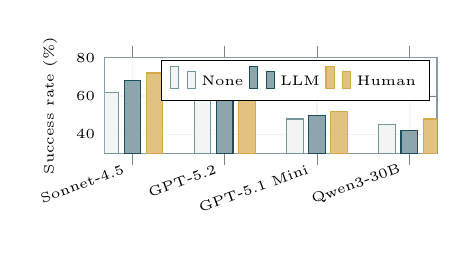
\begin{tikzpicture}
\begin{axis}[
    ybar, bar width=6pt,
    width=5.8cm, height=2.8cm,
    ymin=30, ymax=80,
    ylabel={\tiny Success rate (\%)},
    symbolic x coords={Sonnet-4.5, GPT-5.2, GPT-5.1 Mini, Qwen3-30B},
    xtick=data,
    xticklabel style={font=\tiny, rotate=20, anchor=east},
    yticklabel style={font=\tiny},
    ylabel style={font=\tiny},
    legend style={font=\tiny, at={(0.98,0.98)}, anchor=north east, legend columns=3},
    axis line style={draw=CoolGray},
    grid=major, grid style={draw=CoolGray!12},
]
\addplot[fill=PaleSage!80, draw=SlateTeal!60] coordinates {(Sonnet-4.5,62) (GPT-5.2,65) (GPT-5.1 Mini,48) (Qwen3-30B,45)};
\addplot[fill=SlateTeal!50, draw=SlateTeal] coordinates {(Sonnet-4.5,68) (GPT-5.2,60) (GPT-5.1 Mini,50) (Qwen3-30B,42)};
\addplot[fill=UVMGold!70, draw=UVMGold] coordinates {(Sonnet-4.5,72) (GPT-5.2,63) (GPT-5.1 Mini,52) (Qwen3-30B,48)};
\legend{None, LLM, Human}
\end{axis}
\end{tikzpicture}
\vskip1pt
{\tiny\color{CoolGray} Gloaguen et al.\ (2026), ETH Zurich / INSAIT}
\end{tcolorbox}
\end{column}
\end{columns}
\end{frame}

%% ---- Scope of access / sandboxing ----
\begin{frame}{What It Can Touch --- And How You Widen It}
\vskip2pt
\begin{columns}[T,onlytextwidth]
\begin{column}{0.32\textwidth}
\begin{tcolorbox}[colback=PaleSage, colframe=SlateTeal, boxrule=0.9pt, arc=3pt, left=5pt, right=5pt, top=3pt, bottom=3pt, title={\faFolderOpen\quad 1. Default}, fonttitle=\bfseries\small\color{white}, coltitle=white, colbacktitle=SlateTeal]
\small
\textbf{Your working directory only.}
\vskip3pt
Asks before each action. This is where you start --- and where most work happens.
\end{tcolorbox}
\end{column}
\begin{column}{0.32\textwidth}
\begin{tcolorbox}[colback=LightGold, colframe=UVMGold, boxrule=0.9pt, arc=3pt, left=5pt, right=5pt, top=3pt, bottom=3pt, title={\faKey\quad 2. Widen}, fonttitle=\bfseries\small\color{white}, coltitle=white, colbacktitle=UVMGold]
\small
\textbf{Grant more as trust grows.}
\vskip3pt
More folders, standing permissions for actions you've vetted. You loosen it deliberately.
\end{tcolorbox}
\end{column}
\begin{column}{0.32\textwidth}
\begin{tcolorbox}[colback=PaleSage, colframe=CoolGray, boxrule=0.9pt, arc=3pt, left=5pt, right=5pt, top=3pt, bottom=3pt, title={\faServer\quad 3. Sandbox / VM}, fonttitle=\bfseries\small\color{white}, coltitle=white, colbacktitle=CoolGray]
\small
\textbf{Isolated environment.}
\vskip3pt
For big, autonomous jobs --- let it run freely in a space that \emph{can't} touch the rest of your machine.
\end{tcolorbox}
\end{column}
\end{columns}
\vskip4pt
\begin{center}
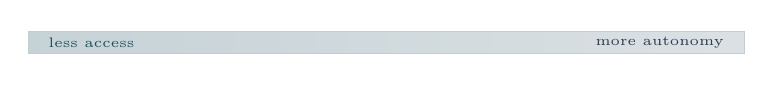
\begin{tikzpicture}[x=0.075\textwidth]
  \shade[left color=SlateTeal!25, right color=CoolGray!30] (0,0) rectangle (10,0.28);
  \draw[CoolGray!50, thin] (0,0) rectangle (10,0.28);
  \node[right, font=\tiny\color{SlateTeal}] at (0.15,0.14) {less access};
  \node[left, font=\tiny\color{DeepCharcoal}] at (9.85,0.14) {more autonomy};
\end{tikzpicture}
\end{center}
\vskip2pt
\begin{columns}[T,onlytextwidth]
\begin{column}{0.62\textwidth}
\begin{tcolorbox}[accentbox, top=3pt, bottom=3pt]
\small \faLock\;\, \textbf{Privacy:} nothing leaves your machine unless you send it. Local files stay local --- you control what it sees.
\end{tcolorbox}
\end{column}
\begin{column}{0.33\textwidth}
\begin{tcolorbox}[colback=SoftCoral!8, colframe=SoftCoral!60, boxrule=0.5pt, arc=3pt, left=5pt, right=5pt, top=3pt, bottom=3pt]
\scriptsize \textbf{\color{SoftCoral}Far beyond this:} full ``god mode'' (email, send, delete). We \textbf{don't} go there.
\end{tcolorbox}
\end{column}
\end{columns}
\end{frame}

%% ---- Your first five minutes (getting-started walkthrough) ----
\begin{frame}[fragile]{Your First Five Minutes}
\vskip2pt
\begin{columns}[T]
\begin{column}{0.52\textwidth}
\begin{tcolorbox}[keybox, title={\faPlay\quad The loop everyone starts with}, top=3pt, bottom=3pt]
\small
\begin{enumerate}\setlength{\itemsep}{4pt}
  \item \textbf{Open it} in your project folder --- type \texttt{claude}
  \item \textbf{Ask} for something small: \textit{``list the files and tell me what this project does''}
  \item It \textbf{asks permission} to act --- you \textbf{grant} it (once)
  \item It asks \textit{again}\ldots and again. \textbf{Annoying.}
  \item Trust it for that action? \textbf{Grant standing permission} (``always allow'')
\end{enumerate}
\end{tcolorbox}
\end{column}
\begin{column}{0.44\textwidth}
\begin{tcolorbox}[accentbox, top=3pt, bottom=3pt]
\small
\textbf{Then: save your preferences.}
\vskip3pt
Conventions, do's \& don'ts, allowed actions live in a \texttt{CLAUDE.md} file --- so you don't re-explain yourself every session.
\end{tcolorbox}
\vskip4pt
\begin{tcolorbox}[quotebox, top=3pt, bottom=3pt]
\scriptsize The permission prompts \emph{are} the guardrail. Loosen them \textbf{as you build trust} --- not on day one.
\end{tcolorbox}
\end{column}
\end{columns}
\end{frame}

%% ---- bootcamp: What real prompts look like ----
\begin{frame}[fragile]{What Real Prompts Look Like}
\begin{tcolorbox}[colback=DarkSlate, colframe=DarkSlate, arc=3pt, left=6pt, right=6pt, top=3pt, bottom=3pt]
{\color{CoolGray}\ttfamily\tiny Simple:\color{white}\tiny\\
Write a Stata do-file that cleans this dataset, labels the variables, and saves a clean version.\\[3pt]
\color{CoolGray}\tiny Data exploration:\color{white}\tiny\\
Read the .dta file. Tell me how many observations per year, what variables we have, and flag anything that looks weird. Restrict to working-age adults 25--64 and drop anyone with zero or missing wages. Do this in Stata.\\[3pt]
\color{CoolGray}\tiny Admin:\color{white}\tiny\\
Extract the deadlines from this document and put them in a table.\\[3pt]
\color{CoolGray}\tiny Correction:\color{white}\tiny\\
Fix the language --- this is a replication exercise showing correlations, not a causal estimate.\\[3pt]
\color{CoolGray}\tiny Advanced:\color{white}\tiny\\
Before writing your score, spawn a research subagent. Search for 2--3 of the most-cited papers referenced in the proposal. For each, summarize: (1) its main finding, and (2) how the proposed study builds on or departs from it.
}
\end{tcolorbox}
\vskip2pt
{\small\color{CoolGray} No special syntax. Just say what you want. Iterate from there.}
\end{frame}

%% ---- bootcamp: When to use it / not ----
\begin{frame}{When to Use It --- and When Not To}
\begin{columns}[T]
\begin{column}{0.47\textwidth}
\begin{tcolorbox}[keybox, title={\faCheck\quad Worth the setup cost}]
\small
\begin{itemize}\setlength{\itemsep}{2pt}
  \item Repetitive tasks you do weekly
  \item Multi-step workflows (data $\rightarrow$ analysis $\rightarrow$ writeup)
  \item Drafting in your voice at scale
  \item Exploring unfamiliar code or data
  \item Anything you'd delegate to an RA
\end{itemize}
\end{tcolorbox}
\end{column}
\begin{column}{0.47\textwidth}
\begin{tcolorbox}[colback=SoftCoral!8, colframe=SoftCoral!50, boxrule=0.5pt, arc=3pt, left=5pt, right=5pt, top=3pt, bottom=3pt, title={\color{SoftCoral}\faTimes\; Not worth it}, fonttitle=\small\bfseries, coltitle=SoftCoral]
\small
\begin{itemize}\setlength{\itemsep}{2pt}
  \item If the task takes \textbf{5 minutes by hand}, just do it by hand
  \item Tasks requiring \textbf{domain judgment} (identification strategy, causal interpretation)
  \item Anything with \textbf{confidential data} you can't share with an API (or strip out)
  \item When you need a \textbf{precise citation} and don't have time to verify
\end{itemize}
\end{tcolorbox}
\end{column}
\end{columns}
\vskip4pt
\begin{tcolorbox}[accentbox, halign=center, width=11cm, top=3pt, bottom=3pt]
\small\bfseries The cost to try: \$20/month + 30 minutes of setup. That's it.
\end{tcolorbox}
\end{frame}

%% ---- bootcamp: What we've used this for ----
\begin{frame}{What We've Actually Used This For}
\begin{columns}[T]
\begin{column}{0.47\textwidth}
\begin{tcolorbox}[keybox, title={\faFlask\quad Research}]
\scriptsize
\begin{itemize}\setlength{\itemsep}{0pt}
  \item Built a replication package --- read do-files, found the dependency chain, wrote the master script
  \item Reproducible balance tables (Stata $\rightarrow$ \LaTeX)
  \item R script to pull IPUMS census data via API
  \item Data dictionary from a messy dataset
  \item Adversarial review of our own paper
  \item Structured literature review with memo
\end{itemize}
\end{tcolorbox}
\end{column}
\begin{column}{0.47\textwidth}
\begin{tcolorbox}[keybox, title={\faChalkboard\quad Teaching \& Workflow}]
\scriptsize
\begin{itemize}\setlength{\itemsep}{0pt}
  \item Course website from scratch (Hugo + GitHub Pages)
  \item Lecture slides in Quarto
  \item Assignment prompts and rubrics from learning goals
  \item Inbox triage: categorizes messages by action needed
  \item Email drafting in our own voice
  \item Hockey schedule emails $\rightarrow$ Google Calendar events
\end{itemize}
\end{tcolorbox}
\end{column}
\end{columns}
\vskip4pt
\begin{tcolorbox}[accentbox, halign=center, width=8cm, top=3pt, bottom=3pt]
\small\bfseries These slides were also made with AI.
\end{tcolorbox}
\end{frame}


%% ====== TWO PRINCIPLES (Emily) ======
\begin{frame}{Getting Started --- Two Principles}
\vskip6pt
\begin{tcolorbox}[keybox, title={\faFlask\quad 1.\ Build in a ``lab'' folder}, top=3pt, bottom=3pt]
\small Nervous? Make a small \textbf{sandbox folder} and experiment there. Nothing important to break --- widen out over time as you build trust.
\end{tcolorbox}
\vskip8pt
\begin{tcolorbox}[keybox, title={\faQuestionCircle\quad 2.\ Learn by doing --- just ask it}, top=3pt, bottom=3pt]
\small Don't know how? \textbf{Ask.} Want it done more efficiently? \textbf{Ask.} It teaches you as you go --- you don't need to know the commands first.
\end{tcolorbox}
\end{frame}

%% ====== VOICE FILE DEMO (Emily) ======
\begin{frame}{Demo: Teach It Your Writing Voice}
\vskip2pt
\begin{columns}[T]
\begin{column}{0.50\textwidth}
\begin{tcolorbox}[keybox, title={\faMicrophone\quad A ``voice file''}]
\small A short file describing \emph{how you write} --- tone, sentence length, habits, what you avoid. The AI reads it and matches your style.
\end{tcolorbox}
\end{column}
\begin{column}{0.46\textwidth}
\begin{tcolorbox}[accentbox]
\small \textbf{Live:} build one from a writing sample $\rightarrow$ then use it on a new task.
\end{tcolorbox}
\end{column}
\end{columns}
\vskip8pt
\begin{tcolorbox}[quotebox, halign=center, top=3pt, bottom=3pt]
\small It runs in a folder, and you just \emph{ask} --- both principles, in one minute.
\end{tcolorbox}
\end{frame}

%% ====== BRIDGE TO THE AUDIT ======
\begin{frame}{So You Can Drive It --- But Can You Trust It?}
\vskip4pt
\small You can now point an agent at your work and direct it. For research, that raises the harder question:
\vskip6pt
\begin{tcolorbox}[coralbox, title={\faExclamationTriangle\quad The real question}, top=3pt, bottom=3pt]
\small A pipeline that \emph{runs} is not a pipeline that's \emph{right}. How do you know the output is correct?
\end{tcolorbox}
\vskip8pt
\begin{tcolorbox}[accentbox, halign=center, top=3pt, bottom=3pt]
\small That's the rest of my time: \textbf{AI as an adversarial reader} --- of your code, and of your paper.
\end{tcolorbox}
\end{frame}

%% ====== SLIDE 2: WHAT I'LL SHOW ======
\begin{frame}{What I'll Show You}
\begin{columns}[T]
\begin{column}{0.52\textwidth}
\vskip4pt
One real project --- a remote-education paper I've been trying to publish --- and two ways I used AI on it:
\vskip6pt
\begin{tcolorbox}[keybox, title={\faCode\quad 1. Audit the code}]
\small Turn 3 years of accumulated do-files into a clean, reproducible replication package --- and find bugs along the way.
\end{tcolorbox}
\vskip4pt
\begin{tcolorbox}[keybox, title={\faSearch\quad 2. Audit the paper}]
\small Adversarial referee-style review \emph{before} resubmitting --- then check it against the real referee reports.
\end{tcolorbox}
\end{column}
\begin{column}{0.42\textwidth}
\begin{tcolorbox}[accentbox]
\small
\textbf{The theme:}
\vskip4pt
AI as a fast, tireless \textbf{adversarial reader} of work you've already done.
\vskip4pt
You stay the expert. It does the mechanical reading and cross-checking --- at a scale and patience you can't match.
\end{tcolorbox}
\vskip4pt
{\scriptsize\color{CoolGray} Erkmen follows: AI at the \textit{front} end --- brainstorming and pressure-testing ideas before you've written anything.}
\end{column}
\end{columns}
\end{frame}

%% ====== SECTION DIVIDER: CODE AUDIT ======
{
\setbeamertemplate{footline}{}
\setbeamercolor{background canvas}{bg=SlateTeal}
\begin{frame}[plain, noframenumbering]
\centering\vfill
{\fontsize{22}{28}\bfseries\selectfont\color{white} Part 1}\\[6pt]
{\color{UVMGold}\rule{5cm}{0.8pt}}\\[6pt]
{\normalsize\color{UVMGold} Auditing a Replication Package}\\[4pt]
{\small\color{PaleSage} Bangladesh Remote Education RCT}
\vfill
\end{frame}
}

%% ====== SLIDE 3: CODE AUDIT — BEFORE ======
\begin{frame}[fragile]{Before: 3 Years of Accumulated Code}
\vskip-4pt
\begin{columns}[T]
\begin{column}{0.47\textwidth}
\begin{tcolorbox}[colback=DarkSlate, colframe=SoftCoral, boxrule=0.8pt, arc=2pt,
  left=4pt, right=4pt, top=3pt, bottom=3pt]
{\color{CoolGray}\ttfamily\tiny
02\_Do files/\\
\hspace{0.6em}01\_master\_5th June 2021.do\\
\hspace{0.6em}03\_vargen\_07sep.do\\
\hspace{0.6em}03\_vargen.do\\
\hspace{0.6em}05\_endline balance\_eb.do\\
\hspace{0.6em}05\_endline balance.do\\
\hspace{0.6em}09\_attrition\_8 July\_e.do\\
\hspace{0.6em}09\_attrition\_8 July.do\\
\hspace{0.6em}...\\
\hspace{0.6em}Archive/ {\color{CoolGray!50}(18 files)}\\
\hspace{0.6em}WB Submission Files/ {\color{CoolGray!50}(14 copies)}
}
\end{tcolorbox}
\end{column}
\begin{column}{0.47\textwidth}
{\small\color{SoftCoral}\textbf{The problems:}}
\vskip3pt
\small
\begin{itemize}\setlength{\itemsep}{2pt}
  \item \textbf{51 do-files} across 4 subdirectories
  \item Master file from \textbf{June 2021} --- 3 years stale
  \item Date-in-filename: \texttt{\_07sep}, \texttt{\_02July1130am}
  \item Author-in-filename: \texttt{\_eb}, \texttt{\_e}
  \item Hardcoded paths --- only runs on my machine
  \item No documentation, no version control
\end{itemize}
\vskip3pt
\begin{tcolorbox}[quotebox, top=2pt, bottom=2pt]
\scriptsize This is \textbf{extremely common} in economics. You probably have a project that looks like this.
\end{tcolorbox}
\end{column}
\end{columns}
\end{frame}

%% ====== SLIDE 4: CODE AUDIT — AFTER ======
\begin{frame}[fragile]{After: One Clean, Reproducible Pipeline}
\vskip-4pt
\begin{columns}[T]
\begin{column}{0.47\textwidth}
{\scriptsize
\setlength{\tabcolsep}{3pt}
\begin{tabular}{>{\raggedright\arraybackslash}m{2.6cm} >{\centering\arraybackslash}m{1.4cm} >{\centering\arraybackslash}m{1.4cm}}
\rowcolor{SlateTeal}
\textcolor{white}{\textbf{Dimension}} & \textcolor{white}{\textbf{Before}} & \textcolor{white}{\textbf{After}} \\[1pt]
\rowcolor{PaleSage}
Do-files & 51 & \textbf{8} \\[1pt]
\rowcolor{white}
Master file & 2021 & Current \\[1pt]
\rowcolor{PaleSage}
Config system & None & Template \\[1pt]
\rowcolor{white}
Version control & None & Git \\[1pt]
\rowcolor{PaleSage}
Documentation & None & Full \\[1pt]
\rowcolor{white}
``Which version?'' & Constant & \textbf{Zero} \\[1pt]
\end{tabular}
}
\vskip3pt
\begin{tcolorbox}[accentbox, top=2pt, bottom=2pt]
\scriptsize \textbf{86 old variants} preserved in Archive/ --- nothing deleted, fully reversible.
\end{tcolorbox}
\end{column}
\begin{column}{0.47\textwidth}
\begin{tcolorbox}[colback=DarkSlate, colframe=DarkSlate, arc=2pt,
  left=4pt, right=4pt, top=2pt, bottom=2pt]
{\color{CoolGray}\ttfamily\tiny
bd-remote-ed/\\
\;code/00\_master\_repo.do\\
\;code/07\_Dofiles\_academic/\\
\;\;\_globals.do, 02\_datagen.do,\\
\;\;03\_vargen.do {\color{UVMGold!70}(THE one)}, ...\\
\;\;Archive/ {\color{CoolGray!50}(86 old)}\\
\;config/config\_local\_template.do\\
\;docs/ \;\;justfile \;\;README.md
}
\end{tcolorbox}
\vskip3pt
\begin{tcolorbox}[quotebox, top=2pt, bottom=2pt]
\scriptsize \textbf{Time:} $\sim$2 Claude Code sessions (a few hours).
\textbf{By hand:} days, minimum.
\end{tcolorbox}
\end{column}
\end{columns}
\end{frame}

%% ====== SLIDE 5: THE $FLAGS BUG ======
\begin{frame}[fragile]{The Bug It Found: A Typo Hiding in Plain Sight}
\vskip-2pt
\begin{tcolorbox}[keybox, title={\faBug\quad The \texttt{\$flags} variable list}, top=2pt, bottom=2pt]
\small
\texttt{\$flags} = 17 missing-value indicators used as controls in \textbf{every regression}. Defined independently in 5 scripts.
\end{tcolorbox}
\vskip3pt
\begin{columns}[T]
\begin{column}{0.47\textwidth}
\begin{tcolorbox}[colback=SoftCoral!8, colframe=SoftCoral, boxrule=0.5pt, arc=2pt, left=5pt, right=5pt, top=3pt, bottom=3pt]
\centering{\small\color{SoftCoral}\textbf{3 of 5 scripts (wrong):}}
\vskip3pt
{\ttfamily\small\color{DeepCharcoal}
... \_f\_c\_engaged \_f\_c\_health\\
\colorbox{SoftCoral!20}{\_c\_child\_work}}
\vskip2pt
{\scriptsize Missing the \texttt{\_f\_} prefix}
\end{tcolorbox}
\end{column}
\begin{column}{0.06\textwidth}
\centering\vskip0.8cm
{\large\color{UVMGold}\faArrowRight}
\end{column}
\begin{column}{0.42\textwidth}
\begin{tcolorbox}[colback=PaleSage, colframe=SlateTeal!50, boxrule=0.5pt, arc=2pt, left=5pt, right=5pt, top=3pt, bottom=3pt]
\centering{\small\color{SlateTeal}\textbf{Correct:}}
\vskip3pt
{\ttfamily\small\color{DeepCharcoal}
... \_f\_c\_engaged \_f\_c\_health\\
\colorbox{PaleSage!50}{\_f\_c\_child\_work}}
\end{tcolorbox}
\end{column}
\end{columns}
\vskip3pt
\begin{tcolorbox}[quotebox, top=2pt, bottom=2pt]
\scriptsize \textbf{Result:} \texttt{\_c\_child\_work} appeared \textit{twice} in regressions; the real missing indicator was left out. Survived 10+ versions across 2+ years. No error, no crash --- just quietly wrong.
\textbf{How AI found it:} cross-referencing every \texttt{global flags} definition across all 51 files.
\end{tcolorbox}
\end{frame}

%% ====== SECTION DIVIDER: PAPER AUDIT ======
{
\setbeamertemplate{footline}{}
\setbeamercolor{background canvas}{bg=SlateTeal}
\begin{frame}[plain, noframenumbering]
\centering\vfill
{\fontsize{22}{28}\bfseries\selectfont\color{white} Part 2}\\[6pt]
{\color{UVMGold}\rule{5cm}{0.8pt}}\\[6pt]
{\normalsize\color{UVMGold} Auditing the Paper}\\[4pt]
{\small\color{PaleSage} Can AI Referee Your Own Work?}
\vfill
\end{frame}
}

%% ====== SLIDE 6: WHAT IS /ECON-AUDIT ======
\begin{frame}[fragile]{What Is \texttt{/econ-audit}?}
\vskip-2pt
\begin{columns}[T]
\begin{column}{0.47\textwidth}
\begin{tcolorbox}[keybox, title={\faSearch\quad An Adversarial Review Skill}, top=3pt, bottom=3pt]
\small
A reusable skill that reads a paper and acts as a \textbf{skeptical referee}.
\vskip3pt
\begin{itemize}\setlength{\itemsep}{1pt}
  \item Reads the full paper (LaTeX, tables, appendix)
  \item Checks identification, power, measurement
  \item Produces a structured audit report
  \item Takes $\sim$60 seconds
\end{itemize}
\end{tcolorbox}
\vskip3pt
\begin{tcolorbox}[colback=DarkSlate, colframe=DarkSlate, arc=2pt,
  left=4pt, right=4pt, top=2pt, bottom=2pt]
{\color{CoolGray}\ttfamily\scriptsize \$ npx skills add eabeam/econ-skills \textbackslash\\
\quad\quad --skill econ-audit}
\end{tcolorbox}
\end{column}
\begin{column}{0.47\textwidth}
\begin{tcolorbox}[accentbox, top=3pt, bottom=3pt]
\small
\textbf{What it checks:}
\vskip3pt
\begin{enumerate}\setlength{\itemsep}{1pt}
  \item \textbf{Identification:} Is the causal claim valid?
  \item \textbf{Statistics:} MHT, power, attrition
  \item \textbf{Measurement:} Are variables measured well?
  \item \textbf{Methodology:} Design consistency
  \item \textbf{Presentation:} Framing, length
\end{enumerate}
\end{tcolorbox}
\end{column}
\end{columns}
\end{frame}

%% ====== SLIDE 7: THE AUDIT OUTPUT (shown from saved run) ======
\begin{frame}[fragile]{Running It on the Paper: 5 Critical, 8 Important, 6 Minor}
\vskip-2pt
\begin{columns}[T]
\begin{column}{0.40\textwidth}
\begin{tcolorbox}[colback=DarkSlate, colframe=CoolGray!40, boxrule=0.5pt, arc=3pt,
  left=6pt, right=6pt, top=5pt, bottom=5pt]
{\color{CoolGray}\ttfamily\small\$\; claude}\\[3pt]
{\color{white}\ttfamily\small /econ-audit main.tex}
\end{tcolorbox}
\vskip4pt
{\scriptsize\color{CoolGray} Output shown is from a saved run --- AI output varies between runs, so I pin the version I'm reasoning about.}
\end{column}
\begin{column}{0.55\textwidth}
\small Three of the critical findings:
\vskip3pt
\begin{tcolorbox}[coralbox, title={\faExclamationTriangle\quad Critical}, top=3pt, bottom=3pt]
\footnotesize
\begin{itemize}\setlength{\itemsep}{2pt}
  \item \textbf{A1 --- Identification:} the mediation claim (info $\rightarrow$ tutoring $\rightarrow$ learning) is not identified.
  \item \textbf{B1--B3 --- Statistics:} no MHT adjustment across domains; headline effect below the MDE; underpowered heterogeneity drives the inequality story.
  \item \textbf{C1 --- Measurement:} differential attrition in the learning sample ($p<0.001$); suggested Lee bounds.
\end{itemize}
\end{tcolorbox}
\end{column}
\end{columns}
\end{frame}

%% ====== SLIDE 8: AI AUDIT VS REAL REFEREES ======
\begin{frame}{AI Audit vs.\ Real Referees: 7 of 10 in $\sim$60 Seconds}
\vskip-2pt
{\scriptsize
\begin{tabular}{>{\raggedright\arraybackslash}m{5.5cm} c >{\raggedright\arraybackslash}m{5.2cm}}
\rowcolor{SlateTeal}
\textcolor{white}{\textbf{Referee Criticism}} & \textcolor{white}{\textbf{AI?}} & \textcolor{white}{\textbf{Notes}} \\[2pt]
\rowcolor{PaleSage}
High attrition \& differential attrition & \textcolor{SlateTeal}{\faCheck} & Flagged as Critical; suggested Lee bounds \\[2pt]
\rowcolor{white}
Results don't tell a coherent story & \textcolor{UVMGold}{\faAdjust} & Caught ID problem, missed internal contradictions \\[2pt]
\rowcolor{PaleSage}
Theoretical model not useful & \textcolor{SlateTeal}{\faCheck} & Flagged --- but recommended \textit{including} it \\[2pt]
\rowcolor{white}
Short intervention duration (4--8 weeks) & \textcolor{SoftCoral}{\faTimes} & Requires field knowledge \\[2pt]
\rowcolor{PaleSage}
Noisy learning measures (8-item phone test) & \textcolor{SlateTeal}{\faCheck} & Strong match; flagged IRT minimums \\[2pt]
\rowcolor{white}
Paper too long and hard to follow & \textcolor{SlateTeal}{\faCheck} & Suggested cutting 20--30\% \\[2pt]
\rowcolor{PaleSage}
Multiple hypothesis testing issues & \textcolor{SlateTeal}{\faCheck} & Aggressive; added winner's curse framing \\[2pt]
\rowcolor{white}
Limited external validity / COVID fatigue & \textcolor{UVMGold}{\faAdjust} & Partial; missed publication landscape \\[2pt]
\rowcolor{PaleSage}
Deviations from pre-analysis plan & \textcolor{SlateTeal}{\faCheck} & Caught the spirit, not the specifics \\[2pt]
\rowcolor{white}
Complex randomization hard to interpret & \textcolor{SlateTeal}{\faCheck} & Strong match \\[2pt]
\end{tabular}
}
\vskip3pt
\begin{tcolorbox}[accentbox, top=2pt, bottom=2pt, width=12cm]
\centering\small \textbf{5 full matches, 2 partial, 1 opposite recommendation, 2 misses.}\\
11 referee reports across 8 journals over 4 years --- vs.\ 60 seconds of AI.
\end{tcolorbox}
\end{frame}

%% ====== SLIDE 9: WHAT THE AI MISSED ======
\begin{frame}{What the AI Missed --- And Why It Matters}
\begin{columns}[T]
\begin{column}{0.47\textwidth}
\begin{tcolorbox}[coralbox, title={\faTimes\quad The Misses}, top=4pt, bottom=4pt]
\small
\begin{itemize}\setlength{\itemsep}{4pt}
  \item \textbf{Short duration:} 4--8 weeks is unusually short for an education RCT. Requires knowing field norms.
  \item \textbf{Internal contradictions:} the data arm raised tutoring \textit{more} than the info arm, yet only info improved learning. Referees caught this; AI didn't.
  \item \textbf{COVID fatigue:} ``we've seen too many of these.'' AI can't read the publication landscape.
\end{itemize}
\end{tcolorbox}
\end{column}
\begin{column}{0.47\textwidth}
\begin{tcolorbox}[quotebox]
\small
\textbf{The opposite advice:}\\[3pt]
The AI recommended \textit{including} the conceptual model. Every referee wanted it \textbf{cut}.
\vskip4pt
Sometimes AI gives exactly the wrong recommendation --- because it lacks field conventions.
\end{tcolorbox}
\vskip4pt
\begin{tcolorbox}[accentbox]
\small
\textbf{Pattern:}\\[2pt]
AI reliably catches \textbf{statistical / econometric} issues.\\[2pt]
AI misses \textbf{field knowledge}, \textbf{within-paper logic checks}, and \textbf{publication strategy}.
\end{tcolorbox}
\end{column}
\end{columns}
\end{frame}

%% ====== SLIDE 10: HONEST TAKEAWAY ======
\begin{frame}{Takeaway: A Very Good Pre-Submission Check}
\begin{columns}[T]
\begin{column}{0.50\textwidth}
\begin{tcolorbox}[keybox, title={\faCheck\quad What It Replaces}]
\small
\begin{itemize}\setlength{\itemsep}{3pt}
  \item The first 80\% of what a careful internal seminar discussant would say
  \item Catches the systematic stuff: identification, power, MHT, attrition
  \item In one minute, not one month
\end{itemize}
\end{tcolorbox}
\end{column}
\begin{column}{0.44\textwidth}
\begin{tcolorbox}[colback=SoftCoral!8, colframe=SoftCoral, boxrule=0.5pt, arc=3pt,
  left=6pt, right=6pt, top=4pt, bottom=4pt]
\small
\textbf{What it doesn't replace:}
\vskip3pt
\begin{itemize}\setlength{\itemsep}{2pt}
  \item Field-specific intuition
  \item ``Does this make sense given what we know about Bangladesh?''
  \item Publication strategy
  \item Colleagues who know your work
\end{itemize}
\end{tcolorbox}
\end{column}
\end{columns}
\vskip8pt
\begin{tcolorbox}[quotebox, width=13cm]
\small \textbf{Code audit:} it found bugs I hadn't found in two years. That alone justified the time.\\[2pt]
\textbf{Paper audit:} run it before you send a paper out. It's free, and it catches the embarrassing stuff.
\end{tcolorbox}
\end{frame}

%% ====== SLIDE 11: HANDOFF + RESOURCES ======
\begin{frame}[fragile]{Try It --- And Over to Erkmen}
\begin{columns}[T]
\begin{column}{0.50\textwidth}
\begin{tcolorbox}[keybox, title={\faRocket\quad What to Try First}]
\small
\begin{enumerate}\setlength{\itemsep}{3pt}
  \item Install \texttt{/econ-audit}, run it on your next submission --- before the referees do.
  \item Point Claude Code at a messy project folder and ask it to audit the structure.
\end{enumerate}
\end{tcolorbox}
\vskip4pt
\begin{tcolorbox}[quotebox, top=3pt, bottom=3pt]
\scriptsize Same principle both times: \textbf{AI does the mechanical reading; you keep the judgment.}
\end{tcolorbox}
\end{column}
\begin{column}{0.47\textwidth}
\begin{tcolorbox}[keybox, title={\faLink\quad Resources}, top=3pt, bottom=3pt]
\small
\begin{itemize}\setlength{\itemsep}{3pt}
  \item Econ skills:\\{\scriptsize\ttfamily github.com/eabeam/econ-skills}
  \item Skills library:\\{\scriptsize\ttfamily skills.sh}
  \item Claude Code docs:\\{\scriptsize\ttfamily docs.anthropic.com/en/docs/claude-code}
\end{itemize}
\end{tcolorbox}
\vskip4pt
{\small\color{SlateTeal} Next: Erkmen on using AI to \textbf{brainstorm and pressure-test research ideas}.}
\end{column}
\end{columns}
\end{frame}

%% ====== CLOSING: RESOURCES + GENEROUS CITATION ======
\begin{frame}[fragile]{Resources \& Credit}
\vskip2pt
\begin{columns}[T]
\begin{column}{0.50\textwidth}
\begin{tcolorbox}[keybox, title={\faLink\quad Go deeper}, top=3pt, bottom=3pt]
\small
\begin{itemize}\setlength{\itemsep}{2pt}
  \item Our work: {\scriptsize\ttfamily thinkingwithagents.github.io}
  \item Econ skills: {\scriptsize\ttfamily github.com/eabeam/econ-skills}
  \item Skills library: {\scriptsize\ttfamily skills.sh}
  \item Claude Code docs: {\scriptsize\ttfamily docs.anthropic.com/claude-code}
\end{itemize}
\end{tcolorbox}
\vskip3pt
\begin{tcolorbox}[accentbox, top=2pt, bottom=2pt]
\scriptsize Slides, links, and the follow-up survey come to your inbox after the session.
\end{tcolorbox}
\end{column}
\begin{column}{0.46\textwidth}
\begin{tcolorbox}[quotebox, title={\faHandsHelping\quad Cite generously}, fonttitle=\bfseries\small, top=3pt, bottom=3pt]
\small These tools make it trivial to remix others' ideas. \textbf{Credit the people you build on} --- it's good scholarship and it grows the field.
\end{tcolorbox}
\vskip3pt
\begin{tcolorbox}[colback=PaleSage, colframe=SlateTeal!40, boxrule=0.5pt, left=5pt, right=5pt, top=3pt, bottom=3pt]
\scriptsize
\textbf{With thanks to:}
\begin{itemize}\setlength{\itemsep}{1pt}
  \item Paul Goldsmith-Pinkham --- ways-to-interact framing
  \item Susam Pal --- the ``three inverse laws'' of AI use
  \item @aniketapanjwani --- the tool-adoption poll
  \item Gloaguen et al.\ (2026) --- the \texttt{AGENTS.md} study
\end{itemize}
\end{tcolorbox}
\end{column}
\end{columns}
\end{frame}


\end{document}
